\section{Reddit Corpus}
To answer our research questions, we chose to use the Reddit corpus. Reddit is a large online internet forum where users are able to discuss a wide array of  topics. To start a discussion, someone submits either a hyperlink or text post. Then, people can reply to these submissions. Users can also reply to the replies to these submissions (and so on). Additionally, users can upvote or downvote both submissions and individual comments. 

In the case of submissions, highly upvoted submissions are more likely to be seen, while highly downvoted submissions are less likely to be seen. Under an individual submission, all comment replies to that submission are sorted by score, and all replies to those comments are sorted by score, and so on. If a comment is sufficiently downvoted, it will be hidden. Hidden comments can still be replied to, upvoted, and downvoted. When a comment receives upvotes and downvotes, it is considered \textit{controversial}.  

Reddit is organized into an infinitely expandable number of smaller forums, normally referred to as subreddits. Each of these subreddits can be about any given topic, general or specific. For instance, it's possible to have a subreddit about science, biology, and genetics. These three subreddits would (or at least could) be completely independent, and they are organized in a flat rather than fashion.

Besides the organizational ways that Reddit is different than Twitter, it is also more homogeneous in its user base. The vast majority of the discussions (and all discussions we examined) are in English. Over half of the users are in the United States, and the majority are fairly young. 

DO WE NEED CITATION FOR LAST SENTENCE?

Our data set consists of approximately two terabytes of Reddit data, ranging from the year 2011 to the year 2014. These comments span every subreddit. 

The goal of analyzing the negative comments is to determine when it is acceptable to have negative sentiment. Obviously, negative sentiment when it comes to armed conflicts is a fairly broad idea. Negative sentiment could potentially include anything from hateful to depressed. Nonetheless, the score unambiguously reflects the community's level of acceptance of that negativity. 

\section{Armed Conflict Database}
From the Armed Conflicts Database developed by International Institute for Strategic Study, we obtain various indexes of armed conflicts around the world \cite{(conflictDB)}. As we are interested in recent armed conflicts, we select the ones that were happening at least in one of the three years from 2012 to 2014. In total, we collected 48 conflicts covering regions including Caribbean and the Americas (4), East Asia and Australasia (8), Europe (4), Middle East and North Africa (7), Russia and Eurasia (5), South Asia (9), and Sub-Saharan Africa (11) (see Fig. 1). In general, there are five types of conflicts from our dataset: criminal violence, ethnic conflict, separatist conflict, territorial conflict, foreign involvement and terrorism. Majority of the conflicts are inherently a combination of more than one types. For example, Xinjiang conflict in China is categorized as ethnic conflict, separatist conflict, and also terrorism. All the armed conflicts have relatively different duration, intensity, as well as number of casualties, refugees, and Internally Displaced People (IDP). The average years of all these armed conflicts worldwide is 23 years.

Caribbean and the Americas (4), East Asia and Australasia (8), Europe (4), Middle East and North Africa (7), Russia and Eurasia (5), South Asia (9), and Sub-Saharan Africa (11)

As we are interested in recent armed conflicts, we select the ones that were happening at least in one of the three years from 2012 to 2014. In total, we collected 48 conflicts covering regions iIn general, there are five types of conflicts from our dataset: criminal violence, ethnic conflict, separatist conflict, territorial conflict, foreign involvement and terrorism. Majority of the conflicts are inherently a combination of more than one types. For example, Xinjiang conflict in China is categorized as ethnic conflict, separatist conflict, and also terrorism. All the armed conflicts have relatively different duration, intensity, as well as number of casualties, refugees, and Internally Displaced People (IDP). The average years of all these armed conflicts worldwide is 23 years.

\begin{figure}
\centering
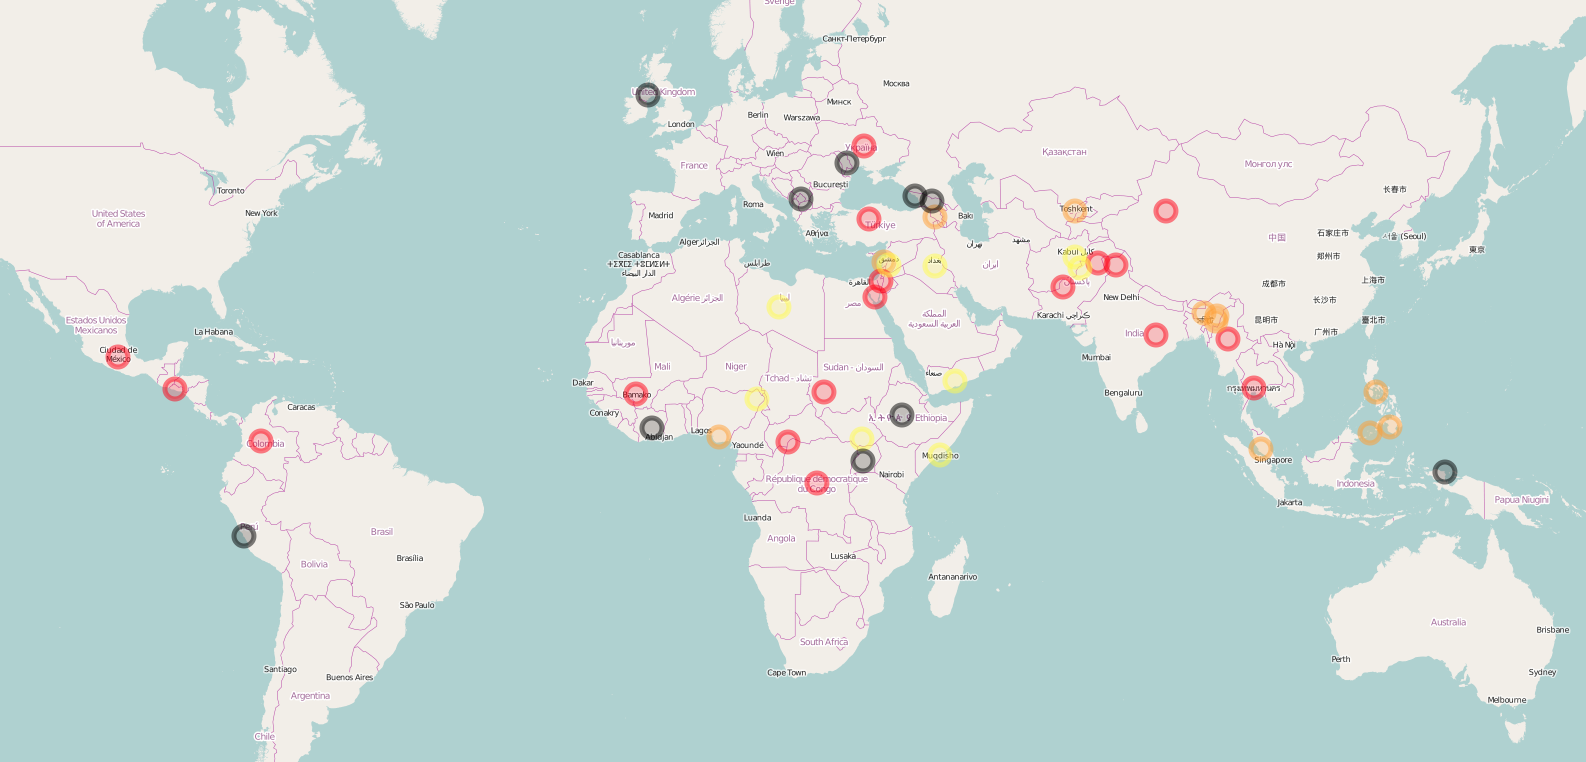
\includegraphics[width=0.9\columnwidth]{map.png}
\caption{A map of 48 conflicts. Black, yellow, orange and red circles indicate the level of intensity: archieved, low, medium and high, respectively.}
\label{rot}
\end{figure}


